
% --------------------------------------------------------------
% This is all preamble stuff that you don't have to worry about.
% Head down to where it says "Start here"
% --------------------------------------------------------------
 
\documentclass[12pt]{article}
 
\usepackage[margin=1in]{geometry} 
\usepackage{amsmath,amsthm,amssymb}
 
\usepackage{listings}
\lstset{
basicstyle=\small\ttfamily,
columns=flexible,
breaklines=true
} 
 
\usepackage{graphics,amsfonts}
\usepackage{epstopdf}
\usepackage[pdftex]{graphicx}
\usepackage{float}
\usepackage{scrextend}
 
\newcommand{\N}{\mathbb{N}}
\newcommand{\Z}{\mathbb{Z}}
 
\newenvironment{theorem}[2][Theorem]{\begin{trivlist}
\item[\hskip \labelsep {\bfseries #1}\hskip \labelsep {\bfseries #2.}]}{\end{trivlist}}
\newenvironment{lemma}[2][Lemma]{\begin{trivlist}
\item[\hskip \labelsep {\bfseries #1}\hskip \labelsep {\bfseries #2.}]}{\end{trivlist}}
\newenvironment{exercise}[2][Exercise]{\begin{trivlist}
\item[\hskip \labelsep {\bfseries #1}\hskip \labelsep {\bfseries #2.}]}{\end{trivlist}}
\newenvironment{reflection}[2][Reflection]{\begin{trivlist}
\item[\hskip \labelsep {\bfseries #1}\hskip \labelsep {\bfseries #2.}]}{\end{trivlist}}
\newenvironment{proposition}[2][Proposition]{\begin{trivlist}
\item[\hskip \labelsep {\bfseries #1}\hskip \labelsep {\bfseries #2.}]}{\end{trivlist}}
\newenvironment{corollary}[2][Corollary]{\begin{trivlist}
\item[\hskip \labelsep {\bfseries #1}\hskip \labelsep {\bfseries #2.}]}{\end{trivlist}}
 
\usepackage{blindtext} % for dummy text

\makeatletter
    \setlength\@fptop{0\p@}
\makeatother

\begin{document}
 
% --------------------------------------------------------------
%                         Start here
% --------------------------------------------------------------
 
%\renewcommand{\qedsymbol}{\filledbox}
 
\title{Homework 3\\
Lab 7:  Machine Learning / Deep Learning}%replace X with the appropriate number
\author{Carlo Rizzardo - 1156404\\ %replace with your name
Computer Vision} %if necessary, replace with your course title
 
\maketitle


To complete the \texttt{CascadeClassifierContainer} class the constructors and the methods \texttt{init()} and \texttt{classify(const cv::Mat \&frame)} had to be implemented.
In the provided solution the constructor just sets up the filename for the classifier xml definition and calls \texttt{init()} which in turn sets up the \texttt{cv::CascadeClassifier} by loading the xml file.
The \texttt{classify(const cv::Mat \&frame)} method performs classification on the provided image and highlights the detected cars by drawing red rectangles on the image.
A minimal preprocessing is done on the image before attempting the detection, first the image is converted to greyscale, then it gets equalized using the opencv \texttt{equalizeHist()} function.
The actual classification is done by the \texttt{CascadeClassifier::detectMultiScale()} method which provides a few parameters to configure the algorithm:
\begin{labeling}{params}
\item[\texttt{scaleFactor}] specifies how much the image is scaled down at each round, and so at which scales the detection is attempted. 1.1 has resulted to be a good value.
\item[\texttt{minNeighbors}] specifies the number of neighboring detections needed to accept the detection as valid. This is meant to avoid false positives but too high values tend to exclude also true detections. Values between 3 and 6 achieve good results.
\item[\texttt{minSize}] defines the minimum size for a detected object. In this case a good value is 30x30.
\item[\texttt{maxSize}] defines the maximum size for a detected object. For this application it can be left to the default value, which doesn't set any maximum limit.
\end{labeling}


The \texttt{cascadeClassifier} has been trained with 16 stages and the parameters suggested in the homework instructions. Weaker trainings with 8 and 12 stages resulted to be inadequate as they caused too many false positives.

The yolo classifier had just one parameter to tweak, the \texttt{yolo\_confidence} argument of the main program. Values between 0.3 and 0.4 yields good results, even if they still produce some false positives.



\begin{figure}[ht!]
	\centering
 	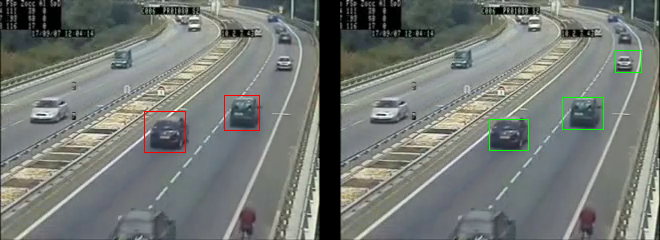
\includegraphics[scale = 0.7]{./frame}
	\caption{ A frame of the resulting video with \texttt{scaleFactor} = 1.1, \texttt{minNeigbors} = 4,\texttt{minSize} = 30x30, \texttt{maxSize} = \texttt{Size()}, \texttt{yolo\_confidence} = 0.3}
\end{figure}
 

\end{document}
              